\documentclass[11pt]{article}
\usepackage[margin=1in]{geometry}
\usepackage{graphicx}
\usepackage{booktabs}
\usepackage{array}
\usepackage{tabularx}
\usepackage{hyperref}
\usepackage{xcolor}
\usepackage{listings}
\usepackage{float}
\usepackage{amsmath}
\usepackage{url}

\hypersetup{
  colorlinks=true,
  linkcolor=blue,
  citecolor=blue,
  urlcolor=blue
}

\lstset{
  basicstyle=\ttfamily\small,
  breaklines=true,
  frame=single,
  columns=fullflexible
}

\title{ML PASS 1 -- Data-Driven SST Correction for NASA Hump}
\author{Codex refinement pass in the local repository workspace}
\date{April 4, 2026}

\begin{document}
\setlength{\emergencystretch}{3em}
\maketitle

\section{Objective}
ML PASS 1 tested a very small, bounded, data-driven correction inside the SST turbulence model for the reconstructed NASA hump case. The goal was not to fit wall curves directly, but to ask whether a physically interpretable correction to the modeled turbulent viscosity could reduce the gap to the official NASA \(C_p\) and \(C_f\) data while also improving the benchmark MAE.

\section{Background}
The pass-four baseline established two important facts:
\begin{itemize}
\item the best honest pass-four result came from deeper convergence of the existing SST setup rather than from a more complicated inlet model;
\item the direct machine-readable NASA \(C_p\) and \(C_f\) comparison pipeline was already in place and should stay central to any later refinement.
\end{itemize}

The pass-four reference target for this experiment remained:
\begin{itemize}
\item benchmark MAE: \texttt{0.1659136747}
\item baseline continuation at \texttt{800} iterations: benchmark MAE \texttt{0.1547381028}
\end{itemize}

\section{Methodology}
\subsection{Baseline SST Setup}
ML PASS 1 reused the pass-four case structure and its existing evaluation pipeline:
\begin{itemize}
\item geometry and mesh generation:
  \path{scripts/generate_nasa_hump_blockmesh.py}
\item case numerics:
  \path{scripts/configure_nasa_hump_case.py}
\item official wall-data evaluation:
  \path{scripts/evaluate_nasa_hump_wall_metrics.py}
\item benchmark MAE evaluation:
  \path{scripts/evaluate_nasa_hump_case.py}
\end{itemize}

The experiment started from the pass-four \texttt{650}-iteration field preserved under \path{data/NASA_2DWMH_backup_before_promotion}. This kept the comparison aligned with the pass-four baseline instead of restarting from scratch.

\subsection{Correction Design}
The custom model added in ML PASS 1 is \texttt{kOmegaSSTML}. It subclasses the standard SST model and applies a bounded multiplicative correction to \(\nu_t\) after the SST model computes its own turbulent viscosity:
\[
f_{corr}
=
\mathrm{clip}\left(1 + A \, g_{\chi}(\nu_t/\nu) \, g_y(y),\; f_{min},\; f_{max}\right)
\]

where:
\begin{itemize}
\item \(A\) is the correction amplitude;
\item \(g_{\chi}\) is a smooth activation based on the eddy-viscosity ratio \(\nu_t/\nu\);
\item \(g_y\) is a Gaussian wall-distance band centered at \(y_{peak}\);
\item \(f_{min}=0.85\) and \(f_{max}=1.60\) keep the correction bounded.
\end{itemize}

This design was chosen because it is:
\begin{itemize}
\item low-dimensional;
\item easy to toggle on or off;
\item physically interpretable as a localized mixing correction;
\item embedded inside the turbulence model rather than added in post-processing.
\end{itemize}

The optimized parameter set was intentionally small:
\begin{itemize}
\item amplitude \(A\)
\item activation threshold \(\chi_0\)
\item wall-distance center \(y_{peak}\)
\end{itemize}

The remaining parameters were fixed:
\begin{itemize}
\item \(\chi\)-activation width \(= 1.0\)
\item wall-band width \(= 0.010\) m
\item \(f_{min}=0.85\)
\item \(f_{max}=1.60\)
\end{itemize}

\subsection{Objective Function}
The scalar objective used in ML PASS 1 was:
\[
J = 0.55 \, \mathrm{MAE} + 0.30 \, C_p\mathrm{MAE} + 0.15 \, \left(C_f\mathrm{MAE}/10^{-3}\right) + P
\]

with regularization:
\[
P = 0.02 \left(\frac{A}{0.6}\right)^2
\]

This keeps the benchmark MAE as the dominant term while still forcing the search to care about direct agreement with the official wall metrics. The penalty discourages unnecessarily strong corrections.

\subsection{Optimizer Choice}
The optimization used \texttt{Nelder-Mead}, which satisfies the no-adjoint and no-gradient requirement. The search budget was deliberately small:
\begin{itemize}
\item cheap stage:
  continue from \texttt{650} to \texttt{720}
\item full stage:
  continue from \texttt{650} to \texttt{800}
\item maximum cheap-stage evaluations:
  \texttt{6}
\end{itemize}

This budget was chosen after an initial higher-cost setup proved unnecessarily expensive for the first ML screening pass.

\section{Optimization Process}
\begin{table}[H]
\centering
\scriptsize
\begin{tabularx}{\linewidth}{>{\raggedright\arraybackslash}p{0.16\linewidth} >{\raggedleft\arraybackslash}p{0.09\linewidth} >{\raggedleft\arraybackslash}p{0.10\linewidth} >{\raggedleft\arraybackslash}p{0.10\linewidth} >{\raggedleft\arraybackslash}p{0.10\linewidth} >{\raggedleft\arraybackslash}p{0.10\linewidth} >{\raggedright\arraybackslash}X}
\toprule
Case & Time & MAE & \(C_p\) MAE & \(C_f\) MAE & Objective & Notes \\
\midrule
Baseline SST & 720 & 0.1604051334 & 0.1676377302 & 0.0008080283 & 0.2597183893 & Cheap-stage reference continuation from the pass-four \texttt{650} field. \\
Baseline SST & 800 & 0.1547381028 & 0.1641787966 & 0.0007681825 & 0.2495869738 & Full-stage reference continuation from the pass-four \texttt{650} field. \\
ML cand. 1 & 720 & 0.1604051334 & 0.1676377302 & 0.0008080283 & 0.2631906115 & \(A=0.25,\chi_0=4.0,y_{peak}=0.015\). \\
ML cand. 2 & 720 & 0.1604051334 & 0.1676377302 & 0.0008080283 & 0.2602739448 & \(A=0.10,\chi_0=3.0,y_{peak}=0.012\). \\
ML cand. 3 & 720 & 0.1604051334 & 0.1676377302 & 0.0008080283 & 0.2665239448 & \(A=0.35,\chi_0=6.0,y_{peak}=0.015\). \\
ML cand. 4 & 720 & 0.1604051334 & 0.1676377302 & 0.0008080283 & 0.2631906115 & \(A=0.25,\chi_0=8.0,y_{peak}=0.020\). \\
ML cand. 5 & 720 & 0.1604051334 & 0.1676377302 & 0.0008080283 & 0.2598572781 & \(A=0.05,\chi_0=3.49,y_{peak}=0.0163\). \\
ML cand. 6 & 720 & 0.1604051334 & 0.1676377302 & 0.0008080283 & 0.2597183893 & Zero-amplitude limit chosen by the optimizer. \\
Best nonzero corrected & 800 & 0.1547381028 & 0.1641787966 & 0.0007681825 & 0.2497258627 & \(A=0.05,\chi_0=3.49,y_{peak}=0.0163\). \\
\bottomrule
\end{tabularx}
\normalsize
\caption{ML PASS 1 objective history and shortlisted full-stage cases.}
\end{table}

\begin{figure}[H]
\centering
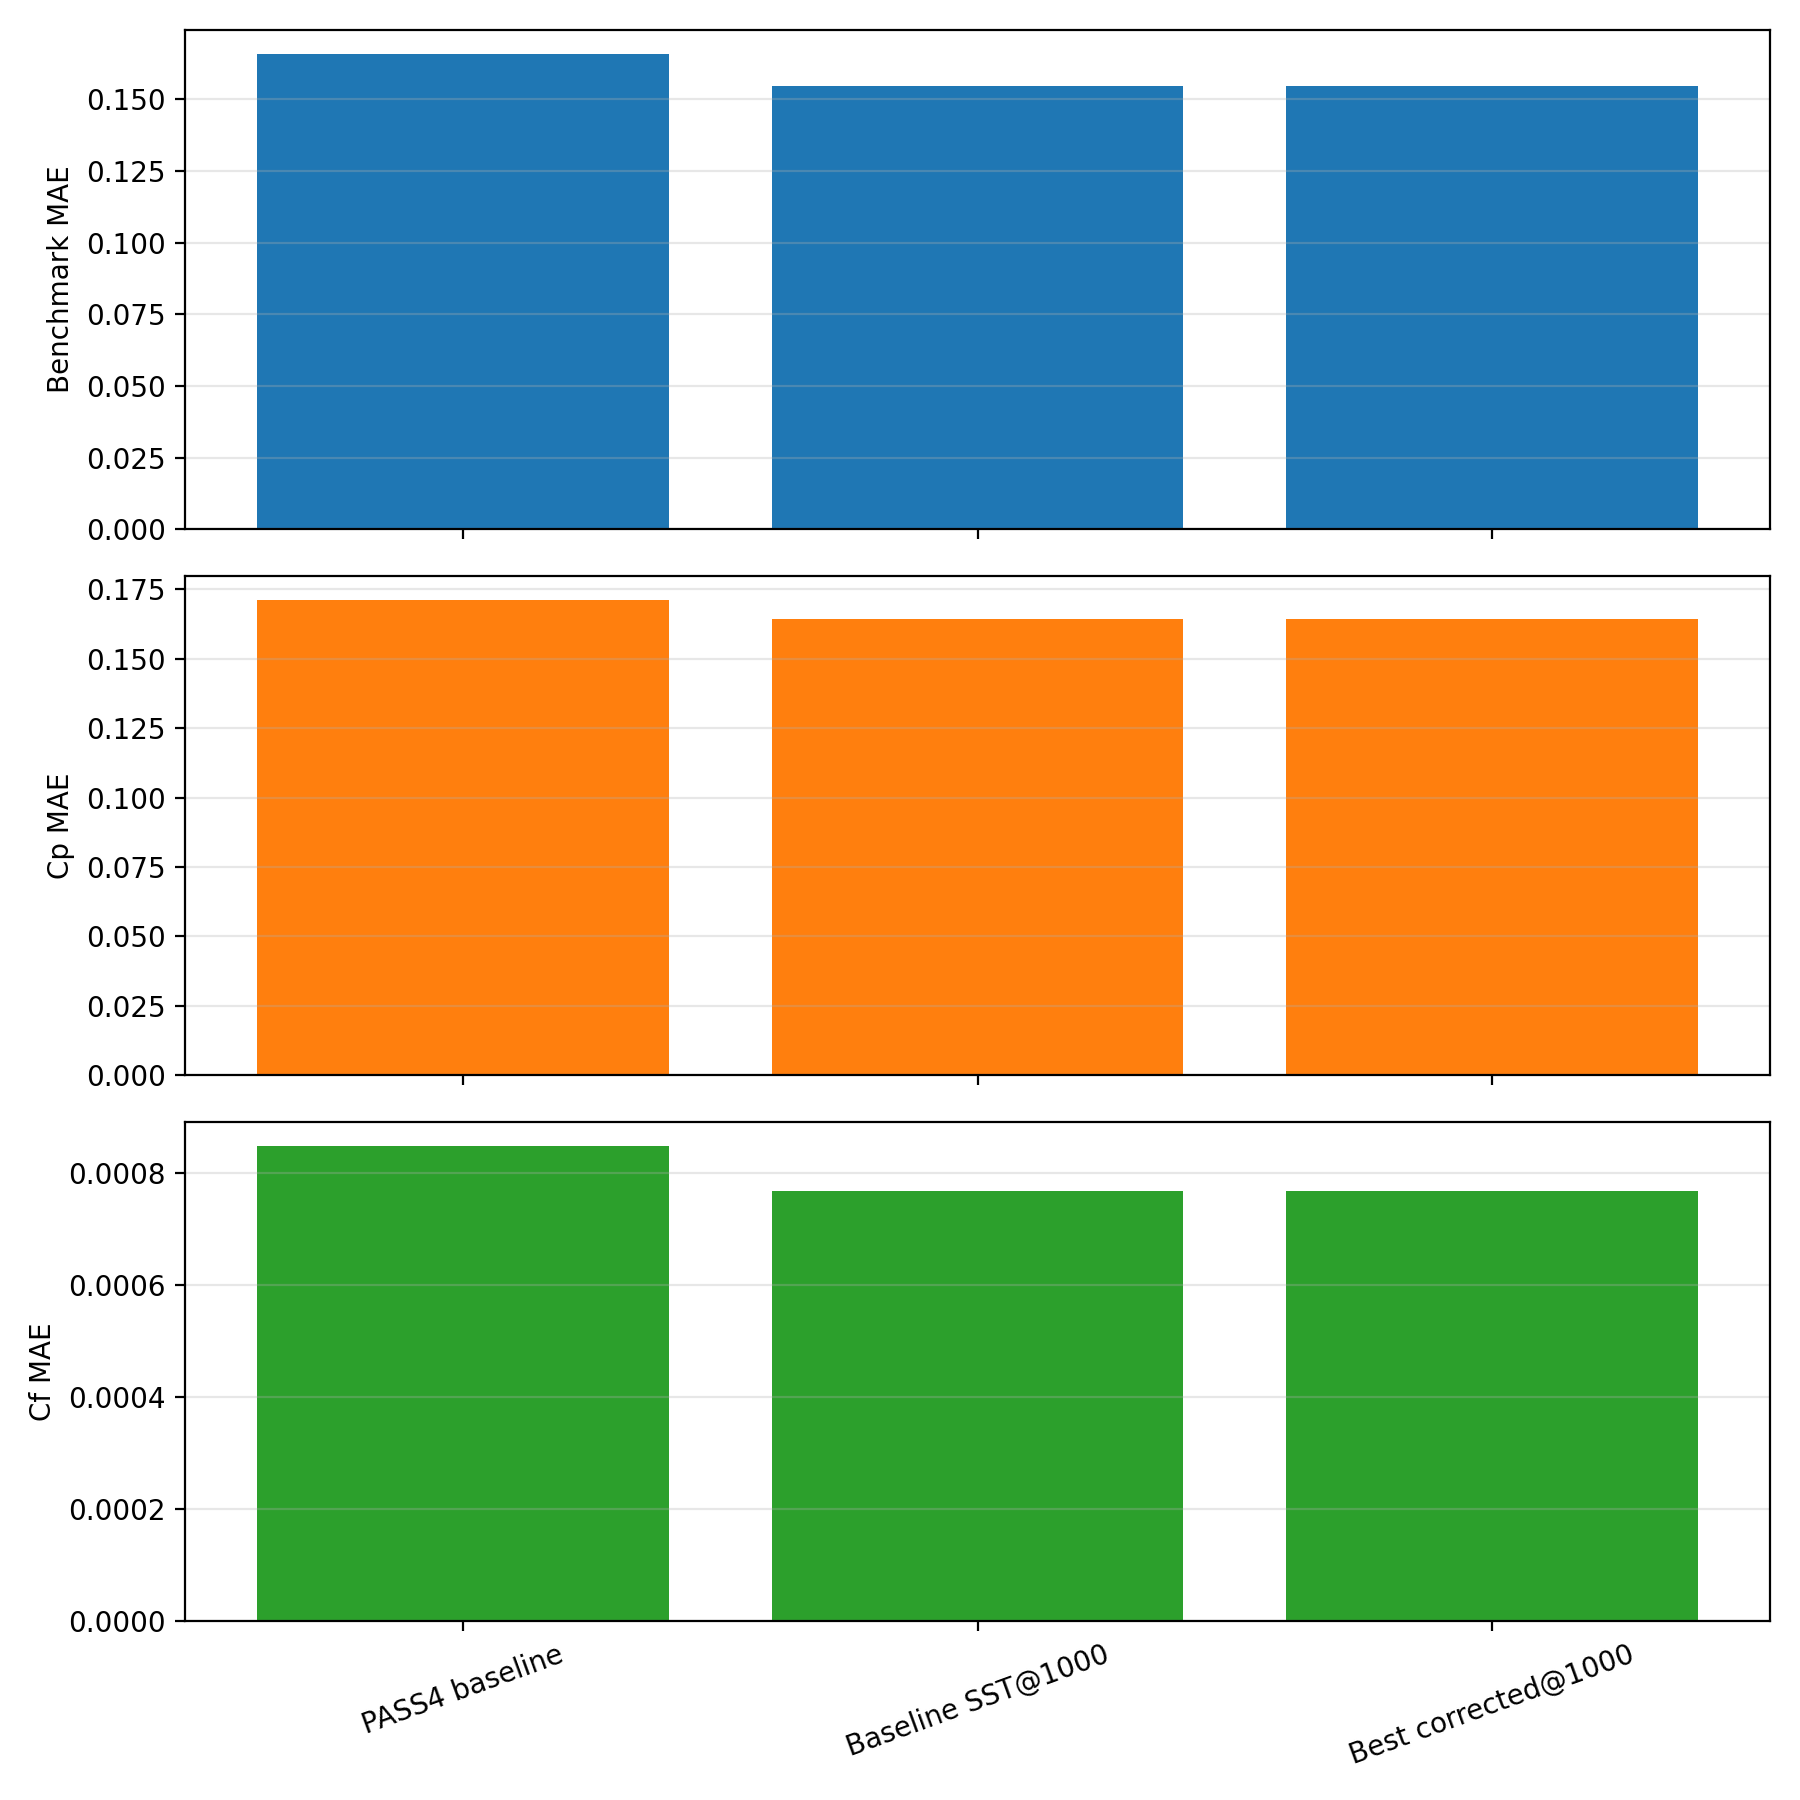
\includegraphics[width=0.94\linewidth]{figures_mlpass1/mlpass1_metric_comparison.png}
\caption{Metric comparison between the pass-four reference, the plain SST continuation, and the best nonzero corrected candidate.}
\end{figure}

\section{Results}
\begin{figure}[H]
\centering
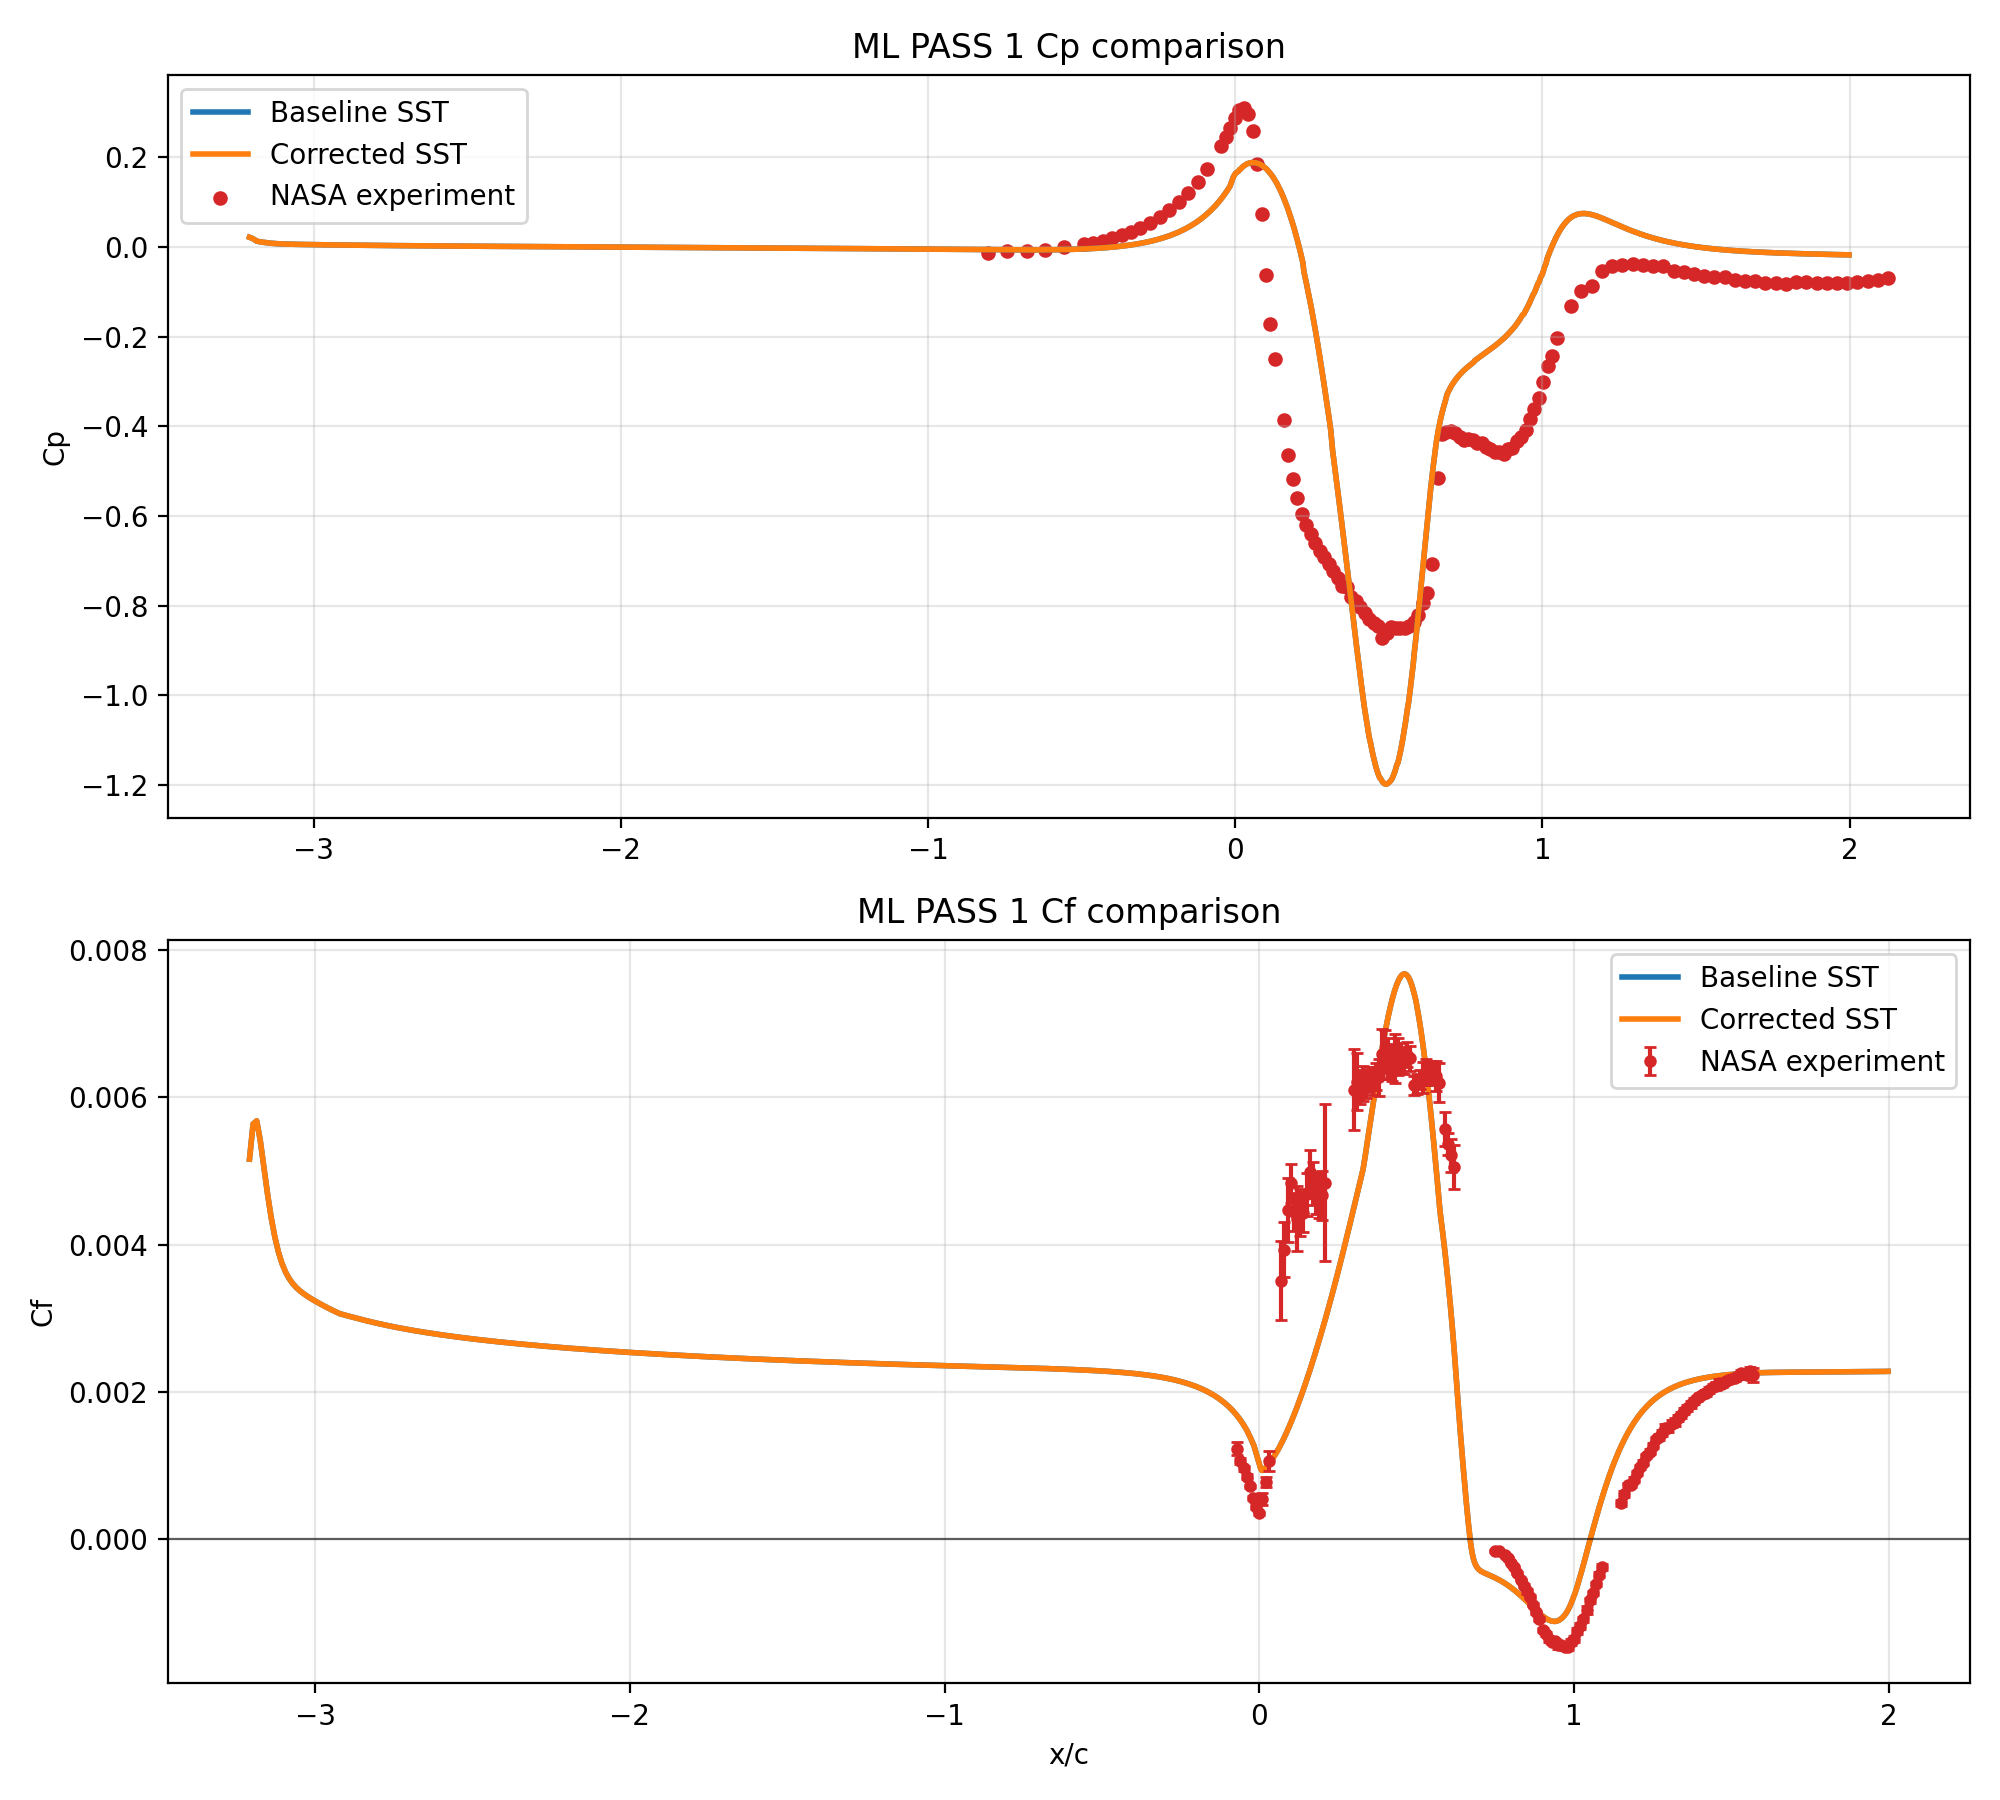
\includegraphics[width=0.94\linewidth]{figures_mlpass1/cp_cf_mlpass1.png}
\caption{Official NASA \(C_p\) and \(C_f\) data compared against the baseline SST continuation and the best nonzero corrected SST candidate.}
\end{figure}

The two decisive observations are:
\begin{itemize}
\item the cheap-stage corrected candidates remained stable, so the correction form was numerically well behaved;
\item none of the nonzero corrections improved the flow metrics relative to the plain SST continuation.
\end{itemize}

The best nonzero corrected full-stage candidate was:
\begin{itemize}
\item amplitude: \texttt{0.05}
\item \(\chi_0\): \texttt{3.4943}
\item \(y_{peak}\): \texttt{0.01633 m}
\item benchmark MAE: \texttt{0.1547381028}
\item \(C_p\) MAE: \texttt{0.1641787966}
\item \(C_f\) MAE: \texttt{0.0007681825}
\end{itemize}

Those values are indistinguishable from the plain SST continuation at the same \texttt{800}-iteration depth, and the nonzero correction is therefore dominated by its regularization penalty.

\section{Discussion}
ML PASS 1 produced a useful result even though it did not produce a promoted new model. The bounded correction was:
\begin{itemize}
\item physically interpretable;
\item implemented inside the turbulence model;
\item reproducible through Dockerized OpenFOAM;
\item numerically stable across the tested parameter range.
\end{itemize}

However, it did not improve the hump flow prediction within this budget. The optimizer responded correctly by moving toward the zero-amplitude limit. That is a strong signal that, for this first correction form and this continuation window:
\begin{itemize}
\item the chosen activation based on wall distance and eddy-viscosity ratio was too weakly coupled to the hump metrics;
\item the dominant error at this stage is still better explained by convergence depth and geometry fidelity than by this simple local \(\nu_t\) multiplier;
\item promoting the corrected model would be harder to defend physically than simply keeping the plain SST continuation.
\end{itemize}

This also reduces the risk of overfitting. Because the correction did not buy a metric improvement, the correct scientific action is to reject it rather than pretending the optimizer found a meaningful data-driven gain.

\section{Conclusion}
ML PASS 1 successfully implemented and tested a controlled, bounded, data-driven SST correction inside OpenFOAM. The custom model compiled, ran stably, and remained fully reproducible. But the best nonzero correction did not improve the benchmark MAE, \(C_p\) agreement, or \(C_f\) agreement relative to the plain SST continuation.

Decision:
\begin{itemize}
\item promote corrected model:
  \textbf{no}
\item keep plain SST continuation as the stronger baseline:
  \textbf{yes}
\end{itemize}

The next best ML path is not to enlarge the optimizer blindly. It is to redesign the correction so it acts on a more discriminating separated-shear-layer signal or a more faithful geometry baseline before spending more CFD budget.

\section{Reproducibility}
From the repository root, the ML PASS 1 workflow is:
\begin{lstlisting}
bash scripts/build_ml_hump_model.sh
bash scripts/run_nasa_hump_mlpass1.sh
MPLCONFIGDIR=docs/.mplconfig python3 scripts/make_nasa_hump_mlpass1_figures.py
bash scripts/build_report.sh
\end{lstlisting}

\bibliographystyle{plain}
\bibliography{references}

\end{document}
